\documentclass[border=5mm]{standalone}
\usepackage{tikz}
\usetikzlibrary{positioning, arrows.meta, shapes.geometric, graphs, graphs.standard}

\begin{document}

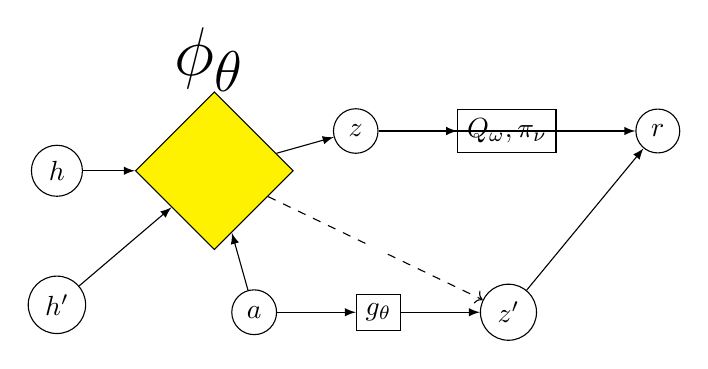
\begin{tikzpicture}[node distance=1cm]
    % Nodes
    \node[circle, draw] (h) {$h$};
    \node[circle, draw, below=of h] (h') {$h'$};
    \node[regular polygon, regular polygon sides=4, minimum size=20mm, rotate=45, fill=yellow, draw] (phi) at (2,0) {};
    \node[circle, draw, right=of phi] (z) {$z$};
    \node[rectangle, draw, right=of z] (q) {$Q_{\omega}, \pi_\nu$};
    \node[circle, draw, right=of q] (r) {$r$};
    \node[circle, draw, below=of phi] (a) {$a$};
    \node[rectangle, draw, right=of a] (g) {$g_\theta$};
    \node[circle, draw, right=of g] (z') {$z'$};

    % Dashed edge for stop-gradient
    \draw[dashed, ->] (phi) -- node[fill=white] {} (z');

    % Edges
    \draw[-latex] (h) -- (phi);
    \draw[-latex] (h') -- (phi);
    \draw[-latex] (phi) -- (z);
    \draw[-latex] (z) -- (q);
    \draw[-latex] (z) -- (r);
    \draw[-latex] (a) -- (phi);
    \draw[-latex] (a) -- (g);
    \draw[-latex] (g) -- (z');
    \draw[-latex] (z') -- (r);

    % Labels
    \node[above=5mm of phi, anchor=south west, inner sep=0pt, outer sep=0pt] {\Huge $\phi_{\theta}$};
\end{tikzpicture}

\textbf{Architecture of our minimalist $\phi_L$ algorithm.} The dashed edge indicates the stop-gradient operator; the undirected edges indicate learning from grounded signals of rewards or next latent states.

\end{document}